
\documentclass[letterpaper, reqno,11pt]{article}
\usepackage[margin=1.0in]{geometry}
\usepackage{color,latexsym,amsmath,amssymb,graphicx,float,hyperref,soul}
\usepackage[dvipsnames]{xcolor}

\usepackage[
backend=biber,
sorting=ynt
]{biblatex-chicago}
\addbibresource{sources.bib}

\newcommand\myshade{85}
\colorlet{mylinkcolor}{violet}
\colorlet{mycitecolor}{orange}
\colorlet{myurlcolor}{Aquamarine}

\hypersetup{
  linkcolor  = mylinkcolor!\myshade!black,
  citecolor  = mycitecolor!\myshade!black,
  urlcolor   = myurlcolor!\myshade!black,
  colorlinks = true,
}
\usepackage{setspace}
\doublespacing

\newcommand{\hlc}[2][yellow]{{%
    \colorlet{foo}{#1}%
    \sethlcolor{foo}\hl{#2}}%
}

\graphicspath{ {images/} }

\begin{document}
\pagenumbering{arabic}
\title{AMNE 151 Final Portfolio}
\date{April 20th, 2023}
\author{Xander Naumenko, 38198354}
\maketitle

\section*{Capstone 4}

{\noindent\bf Prompt: How does this text understand death? What does it tell us about what happens when someone dies?}

\medskip

Someone dying is, to us, intrinsically sad. This fact is so ingrained in our collective morality that it's difficult to interpret stories without this baseline assumption. Upon a careful reading, it may have not been as evident in the ancient Greek psyche\footnote{The metaphysical embodiment of conscious, not the mythological character.}. When discussing sadness pertaining to death, ancient Greek myths consistently focus on aspects of grief quite dissimilar to our modern interpretations.

\medskip

The most candid discussion of death among the primary texts read was, by far, Euripides's {\em Heracles}. During and before Heracles's discussion with Theseus over his inadvertent killing of his family before Theseus arrives, they come to the subject of suicide,\footnote{When Theseus asks what he will do next, Heracles responds ``I will die and return to
that world below from which I have just come.'' \parencite{Euripides} (line 1240)} but the motivation subverts expectations. Instead of Heracles's motivation being the pain he feels for his family's passing, he talks length about how he wishes to end his life to ``avert from [his] life the infamy which now awaits [him].'' \autocite{Euripides} (line 1150) He laments about how his friends will look down on him for his deeds\footnote{When Theseus approaches, he says ``now shall I stand revealed, and the dearest of my friends will see the pollution I have incurred by my children’s murder.''\parencite{Euripides} (line 1155)}, never once mentioning any woe he feels simply for the loss of life of those close to him. In Aeschylus's {\em Prometheus Bound}\autocite{bound} Prometheus echoes a similar sentiment, expressing his desire to cease existence not for his own sadness, but to prevent those around him from looking down at him.\footnote{He says to Hermes ``I wish [Zeus] had hurled me below the earth! Yes beneath Hades, host of the dead, into impenetrable Tartarus, and had bound me ruthlessly there, in unremovable binds, so that no god or human could gloat over my agony!'' \parencite{bound} (line 150) Although not exactly suicide, for a god it seems that Tartarus is the closest equivalent to death.} It's easy to implicitly apply our modern sensibilities to the text and project subtext of sadness onto the conversation, but as read objectively, societal pressure for conformity is what guides their intentions.

\medskip

Of the text's we've read, it would seem that Bion's {\em Lament for Adonis} would completely discredit the thesis discussed so far. The entirety of the poem is dedicated to the sadness of Adonis's passing. However a closer reading reveals a striking fact: the only mention in the text of why his passing is sorrowful is merely the fact it denies Aphrodite his beauty. It even goes so far as to say ``A boar killed the fair man, and it destroyed as well his holy figure. His figure was attractive to Aphrodite, when Adonis was alive, but his beauty is dying away with Adonis. “Alas for Aphrodite!”''\autocite{Bion} This isn't an isolated occurance; Aphrodite missing his beauty is repeated time and time again throughout as the only reason he is worthy to grieve over. The idea of emphasizing the inconvenience of losing a pleasing sexual plaything upon the death of another is unthinkable now. If one were to produce something similar today it would be considered incredibly shallow, but perhaps it simply showcases the differing views ancient Greeks had towards death. This circumstance is complicated by the fact that Aphrodite is a Godess so there's an inherent power imbalance, but perhaps the view of Bion was that it wasn't Adonis's death that was inherently sad, but instead it was the joy he provided to those around him that could no longer occur.

\medskip

The ancient Greek view on death seems to be subtly different than our modern interpretation. Interestingly, they produce similar outcomes; there are many poems today written about people passing away similar to {\em Lament for Adonis}, and Heracle's talk of suicide was surprisingly frank and similar to those contemplating it now. These enduring parallels, despite fundamental differences in morality in as something as omnipresent as death, could potentially be one of the reasons Greek and Roman mythology has retained its pedigree as a bastion of popular culture for countless centuries.

\pagebreak

\section*{Notes on Revisions}

The next three sections are my revised capstone assignments. As requested, I've included both a paragraph explaining my edits as well as footnotes documenting specific changes I made. To make things clear I've distinguished my edits into three categories based on who suggested them with corresponding color: \hlc[Aquamarine]{instructor}, \hlc[BurntOrange]{peer} and \hlc[pink]{self}. Any footnote beginning with one of these documents a non-trivial revision made to what was originally submitted. Given capstone 4 is already on top since it was just written I've put them in reverse chronological order.

\pagebreak

\section*{Capstone 3}

\subsection*{Revision Summary}

This was the capstone I did best on with 88\%, but there were several improvements that I wanted to implement to make my points stronger and more concise. One suggestion from the instructor was to incorporate an image which I thought was a great idea, so I used a primary source image I think very well reflects Atalanta's struggles for recognition. Some areas of my writing were originally overly wordy, so following peer feedback and self reflection I made the concluding paragraph more concise and converted some quotes from being in-line to being in footnotes. This also gave me a bit of room to expand on my interpretation of the image, although given I was a bit over the word count originally I'm still fairly space limited. I thought my overall thesis and arguments were already quite strong, so structurally I kept things similar.

\subsection*{Essay}

{\noindent\bf Hero Choice: Atalanta}

In the abstract, the story of Atalanta is very much that of a stock Greek hero; she is of noble birth, bravely fights the Calydonian Boar and becomes embroiled in god related drama. Despite this, Atalanta is very unlike most other Greek heros in that most of the key conflict within her stories are defined not by external battles with terrible monsters or gods, but by her inspiring struggle with society itself over her place as a woman warrior.

\medskip

This struggle manifests itself within days of being born. After being abandoned by her father for being a girl\footnote{``At birth her father exposed her; he said he wanted sons, not daughters.''\parencite{Aelian}}\footnote{\hlc[pink]{Self}: Moved citation to footnote}, she is then raised by bears and becomes a devotee of Artemis.\footnote{\hlc[pink]{Self}: Reworded section to remove unnecessary text that doesn't advance the thesis} This overt occlusion from the male-glorifying world rears its head once again when she tries to join the Argonauts. It is described how ``she eagerly desired to follow on that quest; but [Jason] of his own accord prevented the maid, for he feared bitter strife on account of her love.''\autocite{Apollonius} Given that she was a disciple of Artemis and her later stories emphasize her virginity it seems likely that such claims of love on Jason's part were based solely on her gender and no small degree of male cockiness. While she eventually does earn the acceptance of her father and her place on the Argonauts, these early foundational struggles have their core conflict intrinsically embedded in her struggle with society for recognition.

\medskip

The immense hardship brought upon society's disdain for an unchangeable part of personal identity isn't something that is characteristic of most Greek heros. Contrast perhaps the most famous myths of Theseus and Atalanta: the Minotaur and the Calydonian Boar respectively. Upon Theseus's success in killing the Minotaur, ``King Minos was so glad that \ldots he sent him home free into his country, giving to him all the other prisoners of Athens.'' \autocite{Plutarch}\footnote{There's no line number's in this text, but it's right at the end in the textbook} Theseus is unambiguously and immediately praised for his feat, there is no question of his background or whether he deserves it. Compare this to when Atalanta helps defeat the Calydonian Boar but receives resentment for a woman receiving its prized skin\footnote{``The sons of Thestios, thinking scorn that a woman should get the prize in the face of men, took the skin from her, alleging that it belonged to them by right.''\parencite{Bibliotheca}}\footnote{\hlc[pink]{Self}: Refactored sentence and brought citation to footnote.} This can even be seen in her representations in ancient artwork such as figure \ref{fig:atalanta}, where she is sidelined as behind the other male heros, and has to spend the second half of the myth fighting for responsibility.\footnote{\hlc[Aquamarine]{Instructor}: Added primary source image and incorporated it into the text.}

\begin{figure}[tpb]
  \centering
  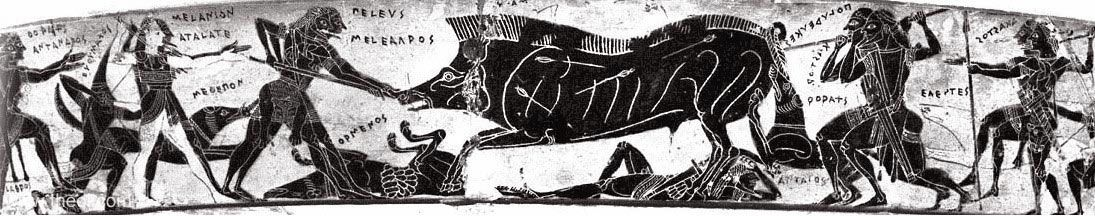
\includegraphics[width=0.8\textwidth]{atalanta}
  \caption{\cite{boar}. Atalanta is pictured third from the left, behind the other male heros actively doing the fighting.}
  \label{fig:atalanta}
\end{figure}


\medskip

For better or for worse, much of Atalanta's mythology is related to her struggles with society to recognize her achievements as that of a woman. It's worth considering though what this tells us about the view that ancient Greek writers had on gender. On one hand, the fact she must contend with men denying her achievements takes space away from the writers emphasizing the heroism of her deeds. It might be meant to leave a Greek listener with the impression that she is notable only for the fact she managed to accomplish challenges as a woman rather than being a great hero who was female. On the other hand though, such a clear story of a woman facing adversity from Greek society and overcoming it is worth telling in its own right. It shows how Greek writers may have understood the path to becoming an independent woman their culture was a long and arduous one, for a mythical hero or not.\footnote{\hlc[BurntOrange]{Peer}: Reworded to avoid overly long and convoluted sentences.}

\pagebreak

\section*{Capstone 2}

\subsection*{Revision Summary}

This was the capstone I was happiest the first time around, so I didn't want to change the structure too much, especially of the story. That being said I originally got an 86\% and I think there are changes that can be made to improve that. When I first wrote it I felt quite constrained by the word count, so I've expanded the story with more details. I thought my analysis was already fairly complete and self contained, so although I've edited it to incorporate feedback, I chose not to expand it just for the sake of filling up space. Most instructor feedback for this essay was positive, so most of the changes were inspired from either self reflection or peer review.

\subsection*{Essay}

{\bf Option 2: Battle Reimagined}

\begin{figure}[h!]
  \centering
  
\includegraphics[width=0.7\textwidth]{im-athena}
  \caption{My image representation of the account. This was made digitally with Midjourney, an AI image generator. The prompt used was ``Athena as president of the united states in front of an american flag, with a staff in her right hand and a shield in her left.'' It is based off the bronze mirror tracing seen in figure \ref{fig:minerva}. It is meant to symbolize how, just as gods have supreme control over the lives of mortals, political power can assert similar influence.}
  \label{fig:im-athena}
\end{figure}

Athena, president of the United States of America, was the last to enter the meeting room. She took stock of the figures arrayed around the table. On her left were the generals, for the most part maintaining a stoic calmness despite the situation. Right were the various government officials, diplomats and ambassadors, displaying a good deal more nervousness about the real possibility of what they were to discuss today.\footnote{\hlc[BurntOrange]{Peer}: Reworded sentences to sound more natural.}

``The Cuban situation must be dealt with.'' Athena stated it not as a query or command, simply as an undeniable truth. ``The United States\footnote{\hlc[pink]{Self}: Fixed capitalization of United States.} has rested too long on our laurels of nuclear supremacy, in the comfortable position to be able to fire missiles from Turkey or Italy at our leisure. That era has come to an end. The Soviets have installed missiles in Cuba, and our diplomatic efforts have yet to bear fruit. We are at a turning point of history. Either we accept the communists as our military equals ad infinitum, or we end it all here with our first strike capabilities. I seek your advice here today to settle this matter.''

She sat down in her chair at the head of the table, while the others in the room uncomfortably looked at one another trying to gauge if she was prompting someone specific to speak. After a few moments the secretary of defense\footnote{\hlc[pink]{Self}: Originally I named him specifically as Robert McNamara, but given no one else in the story was named it sounded quite awkward and I've changed him to unnamed. This isn't based on a fictitious character, in real life he really did advocate for the approach he does here.} spoke up. ``Surely you can't be considering a non-retaliatory strike, Ms. President.''

``Of course she is.'' One of the generals responded, after a few seconds had passed and it was clear that Athena was not willing to engage directly in the conversation. ``They have left us with no choice, we have given the ultimatum after ultimatum, and yet they push us still. If we do not respond while we have the militaristic upper hand, how will we fare when we are on equal footing?''

``Certainly better than the desolated wasteland that we currently know as Europe if we try something so brazen'' the secretary responded. ``We sit here aloof thinking the Soviets are powerless, all the while they have a loaded gun pointed at every single other western power. We like to think fondly back to the time when we were in a position to bomb Japan with impunity, but this isn't the case anymore.''\footnote{\hlc[pink]{Self}: Added this piece of dialogue to better represent the argument against the strike.}

Others hurried to respond, with arguments growing increasingly heated as the evening went on. Athena remained aloof in the discussion, with the full weight of the decision pressing down on her shoulders as she deliberated. After a 3 hours of discussion going around in circles it was clear that everyone in the room, except Athena, had voiced their thoughts. 

``It seems that the time of decision has been reached'' Athena said wearily\footnote{\hlc[BurntOrange]{Peer}: Originally this said ``Athena intoned'', but this fails to convey the difficulty of the choice Athena must make}. ``I appreciate the strategic advice you have given me. Of the non nuclear options, it seems that the defense secretary's plan of naval blockade has the most promise.''

``But that's not enough. I cannot believe in any circumstances that it is a permissible U.S. defensive policy to enable Soviet first strike capabilities. My decision is this: in two days time, we will commence a preemptive nuclear offensive.''

{\bf Explanation of Account}

The account above is a description of a meeting of top government officials during the Cuban Missile Crisis which, while not a traditional battle, was the closest the Cold War came to nuclear war. Based on the primary texts I believe Athena, faced with such the choice of whether to strike first would decide to be the nuclear aggressor.

One might think that as the more strategic counterpart to Ares, Athena would not rush headlong into terrible battle. However Athena's inherent pride in Ovid's {\em Metamorphoses}\autocite{ovid} are a factor pushing her to horrible deeds. In the text she is jealous of Arachne who has her talents\footnote{After Arachne succeeds in her weaving the text states that ``the golden-haired warrior goddess was grieved by [Arachne's] success.''\parencite{ovid}, line 129}. If she resorts to the violence over something as simple as weaving, it's hard to see her allowing another to gain nuclear supremacy alongside her. Just like Arachne taunts Athena with her depictions of Gods' failings\footnote{Arachne's tapestry is ``embroidered with the gods' crimes,'' \parencite{ovid}, line 130, which to make in front of a goddess was clearly a purposeful affront.}, the Soviet Union's continual small transgressions would very possibly push her over the edge.

The strategic sensibility of a first strike would also appeal to the goddess of wisdom. In Homer's {\em Iliad} book 5\autocite{homer}, she is depicted as levelheaded and strategic, unlike Ares. Whereas Ares massacres ruthlessly, Athena hides with Hade's helm of invisibility to strike at Ares in tandem with Diomedes\footnote{In the text ``Athena donned Hade's helmet of invisibility, to hide her identity from the mighty god.''\parencite{homer}, line 845}. A preemptive strike would cost mortal lives, but in the {\em Iliad} Athena was ordering Greeks to battle and ultimately death over the personal insult of a shepherd, so to Athena it's likely the strategic argument would dominate. This is also apparent in the artwork in figure \ref{fig:athena}\autocite{poseidon}. Here Poseidon and Athena are depicted as the center of a grand battle, with their physical size embodying their importance. Those dying in pain around them are markedly smaller, cast by the wayside as pawns in a brutal game of chess.\footnote{\hlc[Aquamarine]{Instructor}: In the rubric evaluation the instructor mentioned the image of Poseidon was fitting but I realized I barely elaborated on it at all, so I added a few sentences in the analysis dedicated to it.}

My image generated with Midjourney\autocite{midjourney}\footnote{There doesn't seem to be a standard way to cite AI image generators currently, so I'm currently just leaving the name and website. I spent quite a while trying to find a definitive source with how to do so with no avail. } is intended to show Athena in a modern light with her traditional symbols combined with the American patriotism behind her pushing her to bold decisions. I wanted to make sure that the artwork represented some aspect of a primary source, so I crafted my prompt similar to a description of figure \ref{fig:minerva}\autocite{minerva}, an early depiction of Athena.\footnote{\hlc[pink]{Self}: Originally this paragraph was quite vague, so I wanted to at least briefly explain my how I created the artwork.}

\begin{figure}[htpb]
  \centering
  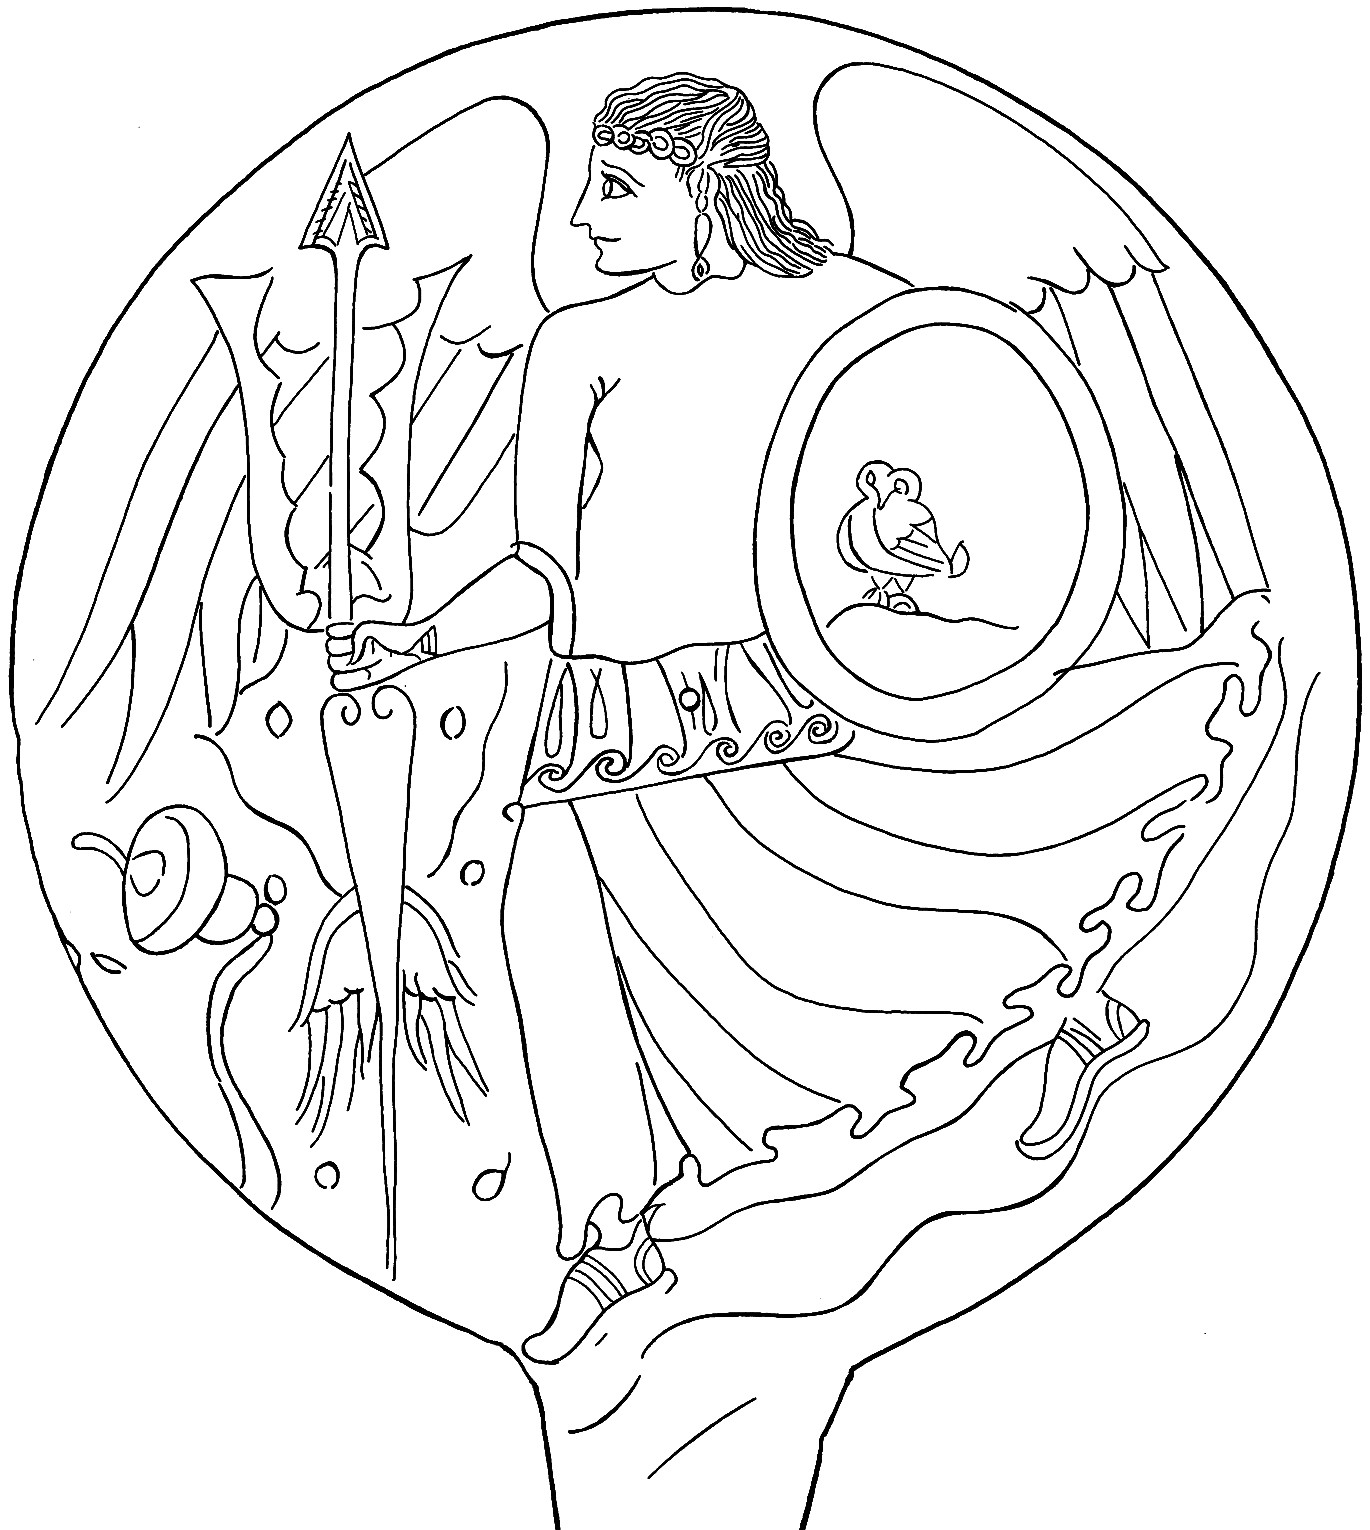
\includegraphics[width=0.5\textwidth]{minerva}
  \caption{\cite{minerva}. An early depiction of what would later become Athena, this is the basis for my generated image seen in figure \ref{fig:im-athena}.}
  \label{fig:minerva}
\end{figure}

\begin{figure}[htpb]
    \centering
    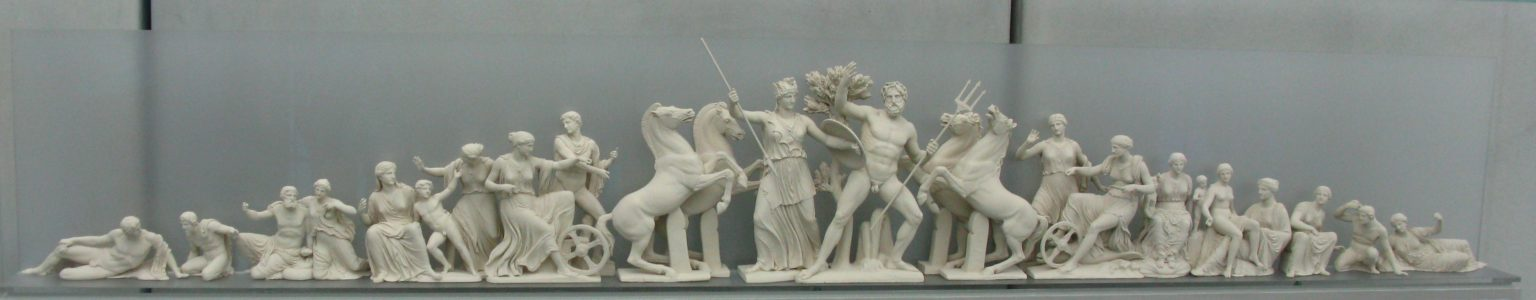
\includegraphics[width=0.8\textwidth]{athena}
    \caption{\cite{poseidon}. A depiction of Athena engaging in a battle of conquest. It seems that the mortals on either side of the gods are suffering from the battle occurring in the middle, but by being depicted as taller it's implied that the Gods' struggles are more relevant. Just like in my account, Athena prioritizes her conquest over the well being of her people.}
    \label{fig:athena}
\end{figure}

\pagebreak

\section*{Capstone 1}

\subsection*{Revision Summary}

This was the capstone I did by far the worst in with a 73\%, so I wanted to revise it fairly heavily to do much better. The biggest thing was to make better use of the primary text. I had originally misinterpreted the capstone requirements, thinking that the intention was for the primary texts to be summarized rather than specific parts used. To correct this I've added in significantly more examples from the text, both in-line and in footnotes. With the increased word count I've also fleshed out my points more thoroughly, as with only 300 words it was difficult to get a clear and sensible argument across. For example I separated the last paragraph into two sections, one focusing on Prometheus and the other on the contrast between him and Pandora, and I completely rewrote the introduction with a hopefully clearer thesis. Finally, I took care of some bookkeeping things that I had neglected before like adding translators to the bibliography.


\subsection*{Essay}

{\bf Prompt:} 2. What does the myth of Pandora tell us about how the ancient Greeks thought about sex/gender and about their views of ancient Greek women? Why is the myth of Prometheus tied to the myth of Pandora?  

\medskip

Both Prometheus and Pandora take actions that have great consequence. Prometheus damns himself to eternal punishment by stealing fire, while Pandora releases misfortune upon the world. However there is a key distinguishing factor between these two events: choice. The myth of Pandora assigns Pandora a distinct lack of agency in her actions compared to Prometheus, and this is representative of the ancient Greek view on their respective genders.\footnote{\hlc[Aquamarine]{Instructor}: Rewrote paragraph to elaborate more and have a more focused thesis}

In Hesiod's \emph{Works and Days} \autocite{works}, it is made clear that Pandora is created to release her slew of evils upon the world.\footnote{It is stated that ``within [Pandora's] breast the messenger and Argos-killer Hermes fashioned lies [pseudea], crafty words, and a sneaky disposition, according to the plans of Zeus the loud-thunderer.'' \parencite{works}} When Zeus gloats over Prometheus he is very upfront about how he will create her specifically for the task: ``As punishment for the fire, I will give them an evil thing, in which they may all take delight, happy in their hearts, embracing this evil thing.''\autocite{works}\footnote{\hlc[BurntOrange]{Peer}: Added supporting quote.} And so while the myth blames Pandora for the many hardships that men face, she was created and deceived into making this choice.\footnote{\hlc[Aquamarine]{Instructor}: Removed ``fluff'' from sentence as per rubric suggestion.} It would be like asking someone if they'd like to sleep on a feather bed or hot spikes without context, then when the bed is obviously selected complaining about how people are too reliant on modern comforts. In this same way giving Pandora the illusion of choice to open the urn without knowledge of the stakes doesn't reflect any agency on Pandora's part. Given that Pandora is the first human woman, she seems to be emblematic of the ancient Greek view on the female gender as a whole. From this viewpoint they didn't think that evil women did chose bad things, it was simply that women were created with some degree of intrinsic wickedness.\footnote{\hlc[pink]{Self}: Rewrote end of this paragraph to better convey point.}

This is especially contrasting to the Prometheus, the reason for Pandora's creation. In Aeschylus's \emph{Prometheus Bound}\autocite{bound}, Prometheus is extremely accepting of the fact that he had full knowledge of his actions' consequences and made the choices he did regardless. When he speaks to Chorus about how he stole fire for humanity and how as a result he was chained to the rocks, he says ``I knew all along what would happen. I did it anyway– I don’t deny it.''\autocite{bound} (Line 265) Unlike Pandora Prometheus was personally responsible for his choices that had a huge impact on humanity, and he is praised for it.His dialogues in {\em Prometheus Bound} present him as a likable, reasonable person coming to terms with his suffering. When he says ``I am a miserable plaything for the wind, and my suffering delights my enemies.''\autocite{bound} (line 155), it is difficult not to sympathize with his plight.\footnote{\hlc[pink]{Self}: Added another quote and elaboration.} Meanwhile Pandora doesn't get a single line of dialogue in any of the works we've seen, despite playing a major role in several.\footnote{\hlc[BurntOrange]{Peer}: Converted this paragraph into two (this one and the next), as these are two distinct ideas.}

This contrast is fitting given Pandora and Prometheus play opposite roles in the same story; Prometheus is the punished and Pandora is the punishment. In this lens Prometheus can be seen as representative of the Greek view on men where they had agency to decide the trajectory of their life, whereas women were denied these choices. That's not to say that women did not play a role in myths. Even discounting goddesses, there have been plenty of women such as Medea and Atalanta\footnote{See capstone 3.} that play major roles. But generally Greek writers put them in the background, with the plot mostly being driven by men making the decisions which reflects the societal view of the time.\footnote{\hlc[Aquamarine]{Instructor}: Expanded this section based on instructor feedback saying that this more of this type of analysis would be appropriate.}

\pagebreak

\printbibliography

\end{document}
